\subsection{Jeu mobile}
Tout d'abord, nous avions besoin d'un jeu non coopératif dans lequel il est possible, à tout moment, de connaître le joueur en tête et de borner la durée d'un niveau. Ces critères peuvent s'adapter à de nombreux types de jeu, comme, par exemple, des jeux de courses, de combat ou bien, dans notre cas, de musique.

Une forme classique de ce type de jeu consiste en un jeu de rythme avec un écran formé de 4 zones verticales. Dans ces zones, des objectifs défilent en descendant et doivent être touchées par le joueur lorsqu'elles arrivent sur une ligne horizontale en bas de l'écran. Les objectifs représentent des notes de musiques qui doivent être jouées au bon moment afin de suivre la bande son du niveau.

\begin{figure}[h]
\begin{center}
\fbox{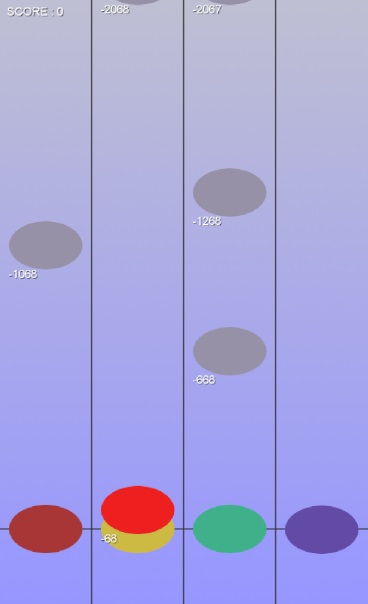
\includegraphics[scale=0.5]{images/jeu3.jpg}}
\end{center}
\caption{Jeu mobile}
\end{figure}

Un niveau se résume à une liste de zones (0,1,2,3) qui est associée à une liste d'instants, à une durée et à une bande son.

Une fois le niveau lancé, le jeu se chargera d'afficher les objectifs au bons endroits en tenant compte du temps écoulé depuis le début du niveau.

Nous avions pensé qu'il pourrait être intéressant de se renseigner sur la possibilité de générer (peut-être partiellement) un niveau de ce jeu à l'aide d'une musique et d'outils d'analyse musicale. Cette idée a finalement été mise à l'écart pour sa difficulté et ne trouvait pas sa place dans le problème posé par le projet.

